\documentclass{ximera}

 

\usepackage{epsfig}

\graphicspath{
  {./}
  {figures/}
}

\usepackage{morewrites}
\makeatletter
\newcommand\subfile[1]{%
\renewcommand{\input}[1]{}%
\begingroup\skip@preamble\otherinput{#1}\endgroup\par\vspace{\topsep}
\let\input\otherinput}
\makeatother

\newcommand{\includeexercises}{\directlua{dofile("/home/jim/linearAlgebra/laode/exercises.lua")}}

%\newcounter{ccounter}
%\setcounter{ccounter}{1}
%\newcommand{\Chapter}[1]{\setcounter{chapter}{\arabic{ccounter}}\chapter{#1}\addtocounter{ccounter}{1}}

%\newcommand{\section}[1]{\section{#1}\setcounter{thm}{0}\setcounter{equation}{0}}

%\renewcommand{\theequation}{\arabic{chapter}.\arabic{section}.\arabic{equation}}
%\renewcommand{\thefigure}{\arabic{chapter}.\arabic{figure}}
%\renewcommand{\thetable}{\arabic{chapter}.\arabic{table}}

%\newcommand{\Sec}[2]{\section{#1}\markright{\arabic{ccounter}.\arabic{section}.#2}\setcounter{equation}{0}\setcounter{thm}{0}\setcounter{figure}{0}}

\newcommand{\Sec}[2]{\section{#1}}

\setcounter{secnumdepth}{2}
%\setcounter{secnumdepth}{1} 

%\newcounter{THM}
%\renewcommand{\theTHM}{\arabic{chapter}.\arabic{section}}

\newcommand{\trademark}{{R\!\!\!\!\!\bigcirc}}
%\newtheorem{exercise}{}

\newcommand{\dfield}{{\sf dfield9}}
\newcommand{\pplane}{{\sf pplane9}}

\newcommand{\EXER}{\section*{Exercises}}%\vspace*{0.2in}\hrule\small\setcounter{exercise}{0}}
\newcommand{\CEXER}{}%\vspace{0.08in}\begin{center}Computer Exercises\end{center}}
\newcommand{\TEXER}{} %\vspace{0.08in}\begin{center}Hand Exercises\end{center}}
\newcommand{\AEXER}{} %\vspace{0.08in}\begin{center}Hand Exercises\end{center}}

% BADBAD: \newcommand{\Bbb}{\bf}

\newcommand{\R}{\mbox{$\Bbb{R}$}}
\newcommand{\C}{\mbox{$\Bbb{C}$}}
\newcommand{\Z}{\mbox{$\Bbb{Z}$}}
\newcommand{\N}{\mbox{$\Bbb{N}$}}
\newcommand{\D}{\mbox{{\bf D}}}
\usepackage{amssymb}
%\newcommand{\qed}{\hfill\mbox{\raggedright$\square$} \vspace{1ex}}
%\newcommand{\proof}{\noindent {\bf Proof:} \hspace{0.1in}}

\newcommand{\setmin}{\;\mbox{--}\;}
\newcommand{\Matlab}{{M\small{AT\-LAB}} }
\newcommand{\Matlabp}{{M\small{AT\-LAB}}}
\newcommand{\computer}{\Matlab Instructions}
\newcommand{\half}{\mbox{$\frac{1}{2}$}}
\newcommand{\compose}{\raisebox{.15ex}{\mbox{{\scriptsize$\circ$}}}}
\newcommand{\AND}{\quad\mbox{and}\quad}
\newcommand{\vect}[2]{\left(\begin{array}{c} #1_1 \\ \vdots \\
 #1_{#2}\end{array}\right)}
\newcommand{\mattwo}[4]{\left(\begin{array}{rr} #1 & #2\\ #3
&#4\end{array}\right)}
\newcommand{\mattwoc}[4]{\left(\begin{array}{cc} #1 & #2\\ #3
&#4\end{array}\right)}
\newcommand{\vectwo}[2]{\left(\begin{array}{r} #1 \\ #2\end{array}\right)}
\newcommand{\vectwoc}[2]{\left(\begin{array}{c} #1 \\ #2\end{array}\right)}

\newcommand{\ignore}[1]{}


\newcommand{\inv}{^{-1}}
\newcommand{\CC}{{\cal C}}
\newcommand{\CCone}{\CC^1}
\newcommand{\Span}{{\rm span}}
\newcommand{\rank}{{\rm rank}}
\newcommand{\trace}{{\rm tr}}
\newcommand{\RE}{{\rm Re}}
\newcommand{\IM}{{\rm Im}}
\newcommand{\nulls}{{\rm null\;space}}

\newcommand{\dps}{\displaystyle}
\newcommand{\arraystart}{\renewcommand{\arraystretch}{1.8}}
\newcommand{\arrayfinish}{\renewcommand{\arraystretch}{1.2}}
\newcommand{\Start}[1]{\vspace{0.08in}\noindent {\bf Section~\ref{#1}}}
\newcommand{\exer}[1]{\noindent {\bf \ref{#1}}}
\newcommand{\ans}{}
\newcommand{\matthree}[9]{\left(\begin{array}{rrr} #1 & #2 & #3 \\ #4 & #5 & #6
\\ #7 & #8 & #9\end{array}\right)}
\newcommand{\cvectwo}[2]{\left(\begin{array}{c} #1 \\ #2\end{array}\right)}
\newcommand{\cmatthree}[9]{\left(\begin{array}{ccc} #1 & #2 & #3 \\ #4 & #5 &
#6 \\ #7 & #8 & #9\end{array}\right)}
\newcommand{\vecthree}[3]{\left(\begin{array}{r} #1 \\ #2 \\
#3\end{array}\right)}
\newcommand{\cvecthree}[3]{\left(\begin{array}{c} #1 \\ #2 \\
#3\end{array}\right)}
\newcommand{\cmattwo}[4]{\left(\begin{array}{cc} #1 & #2\\ #3
&#4\end{array}\right)}

\newcommand{\Matrix}[1]{\ensuremath{\left(\begin{array}{rrrrrrrrrrrrrrrrrr} #1 \end{array}\right)}}

\newcommand{\Matrixc}[1]{\ensuremath{\left(\begin{array}{cccccccccccc} #1 \end{array}\right)}}



\renewcommand{\labelenumi}{\theenumi)}
\newenvironment{enumeratea}%
{\begingroup
 \renewcommand{\theenumi}{\alph{enumi}}
 \renewcommand{\labelenumi}{(\theenumi)}
 \begin{enumerate}}
 {\end{enumerate}\endgroup}



\newcounter{help}
\renewcommand{\thehelp}{\thesection.\arabic{equation}}

%\newenvironment{equation*}%
%{\renewcommand\endequation{\eqno (\theequation)* $$}%
%   \begin{equation}}%
%   {\end{equation}\renewcommand\endequation{\eqno \@eqnnum
%$$\global\@ignoretrue}}

%\input{psfig.tex}

\author{Martin Golubitsky and Michael Dellnitz}

%\newenvironment{matlabEquation}%
%{\renewcommand\endequation{\eqno (\theequation*) $$}%
%   \begin{equation}}%
%   {\end{equation}\renewcommand\endequation{\eqno \@eqnnum
% $$\global\@ignoretrue}}

\newcommand{\soln}{\textbf{Solution:} }
\newcommand{\exercap}[1]{\centerline{Figure~\ref{#1}}}
\newcommand{\exercaptwo}[1]{\centerline{Figure~\ref{#1}a\hspace{2.1in}
Figure~\ref{#1}b}}
\newcommand{\exercapthree}[1]{\centerline{Figure~\ref{#1}a\hspace{1.2in}
Figure~\ref{#1}b\hspace{1.2in}Figure~\ref{#1}c}}
\newcommand{\para}{\hspace{0.4in}}

\renewenvironment{solution}{\suppress}{\endsuppress}

\ifxake
\newenvironment{matlabEquation}{\begin{equation}}{\end{equation}}
\else
\newenvironment{matlabEquation}%
{\let\oldtheequation\theequation\renewcommand{\theequation}{\oldtheequation*}\begin{equation}}%
  {\end{equation}\let\theequation\oldtheequation}
\fi

\makeatother


\title{Matrix Mappings}

\begin{document}
\begin{abstract}
\end{abstract}
\maketitle

  \index{matrix!mappings} \label{s:4.2}

Having illustrated the notational advantage of using matrices
and matrix multiplication, we now begin to discuss why there
is also a {\em conceptual advantage\/} to matrix
multiplication, a conceptual advantage that will help
us to understand how systems of linear equations and linear
differential equations may be solved.

Matrix multiplication allows us to view $m\times n$ matrices as
mappings from $\R^n$ to $\R^m$.  Let $A$ be an $m\times n$
matrix and let $x$ be an $n$ vector.  Then
\[
x \mapsto Ax
\]
defines a mapping from $\R^n$ to $\R^m$.

The simplest example of a matrix mapping is given by $1\times 1$
matrices.  Matrix mappings defined from $\R\to\R$ are
\[
x \mapsto ax
\]
where $a$ is a real number.  Note that the graph of this
function is just a straight line through the origin (with slope
$a$).  From this example we see that matrix mappings are very
special mappings indeed. In higher dimensions, matrix mappings
provide a richer set of mappings; we explore here {\em planar\/}
mappings\index{planar mappings} --- mappings of the plane into
itself --- using \Matlab graphics and the program {\sf map}.

The simplest planar matrix mappings are the
{\em dilatations\/}\index{dilatation}.
Let $A=cI_2$ where $c>0$ is a scalar.  When $c<1$ vectors are
contracted by a factor of $c$ and and these mappings are
examples of {\em contractions}\index{contraction}.
When $c>1$ vectors are
stretched or expanded by a factor of $c$ and these dilatations
are examples of {\em expansions}\index{expansion}.
We now explore some more complicated planar matrix mappings.

The next planar motions that we study are those given by the
matrices
\[
A=\mattwo{\lambda}{0}{0}{\mu}.
\]
Here the matrix mapping is given by $(x,y)\mapsto(\lambda x,\mu y)$;
that is, a mapping that independently stretches and/or contracts the
$x$ and $y$ coordinates.  Even these simple looking mappings can move 
objects in the plane in a somewhat complicated fashion.

\subsection*{The Program {\sf map}}  \index{\computer!map}

We use \Matlab to explore planar matrix mappings 
using the program {\tt map}.  In \Matlab type the command
\begin{verbatim}
map
\end{verbatim}
and a window appears labeled {\sf Map}.  The $2\times 2$ matrix
\begin{equation}. \label{e:map_A}
\mattwo{0}{-1}{1}{0}
\end{equation}
has been pre-entered.  Click on the {\sf Custom} button. In 
the {\sf Icons} menu click on an icon --- say {\sf Dog} --- and 
a blue `{\sf Dog}' will appear in the graphing window. \index{\computer!dog}
Next click on the {\sf Iterate} button and a new version of the {\sf Dog} will
appear in yellow ---the yellow {\sf Dog} is just rotated about
the origin counterclockwise by $90^\circ$ from the blue dog.
Indeed, the matrix \eqref{e:map_A} rotates the plane counterclockwise
by $90^\circ$.  To verify this statement click on {\sf Iterate}
again and see that the yellow dog rotates $90^\circ$
counterclockwise into the magenta dog.  Of course, the magenta
dog is rotated $180^\circ$ from the original blue dog.
Clicking on {\sf Iterate} once more produces a fourth dog --- this one
in cyan.  Finally, one more click on the {\sf Iterate} button will
rotate the cyan dog into a red dog that exactly covers the
original blue dog.

Other matrices will produce different motions of the plane.  Click 
on the {\sf Reset} button.  Then either push the {\sf Custom} button,  
type the entries in the matrix, and click on the {\sf Iterate} button; 
or choose one of the pre-assigned matrices listed in the {\sf Gallery} menu
and click on the {\sf Iterate} button.  
For example, clicking on the {\sf Contracting rotation} button recalls the matrix
\[
\mattwo{0.3}{-0.8}{0.8}{0.3}
\]
This matrix rotates the plane through an angle of approximately
$69.4^\circ$ counterclockwise and contracts the plane by a
factor of approximately $0.85$.  Now click on {\sf Dog} in the
{\sf Icons} menu to bring up the blue dog again.  Repeated
clicking on {\sf Iterate} rotates and contracts the dog so that dogs
in a cycling set of colors slowly converge towards the origin in
a spiral of dogs.\footnote{When using the program {\sf map} first 
choose an Icon (or Vector), second choose a Matrix from the Gallery 
(or a Custom matrix), and finally click on {\sf Iterate}. Then {\sf Iterate} 
again or {\sf Reset} to start over.}

\subsubsection*{Rotations}\index{rotation}

Rotating the plane counterclockwise through an angle $\theta$ is
a motion given by a matrix mapping.  We show that the matrix that
performs this rotation is:
\begin{equation} \label{e:rotmat}
R_\theta = \mattwo{\cos\theta}{-\sin\theta}{\sin\theta}{\cos\theta}.
\end{equation}
To verify that $R_\theta$ rotates the plane counterclockwise
through angle $\theta$, let $v_\varphi$ be the unit vector whose
angle from the horizontal is $\varphi$; that is,
$v_\varphi=(\cos\varphi,\sin\varphi)$.  We can write every vector in
$\R^2$ as $rv_\varphi$ for some number $r\ge 0$.   Using the 
trigonometric identities for the cosine and sine of the sum of two angles, we
have:
\begin{eqnarray*}
R_\theta (rv_\varphi) & = &
\mattwo{\cos\theta}{-\sin\theta}{\sin\theta}{\cos\theta}
\vectwo{r\cos\varphi}{r\sin\varphi} \\
& = & \vectwo{r\cos\theta\cos\varphi -r\sin\theta\sin\varphi}
{r\sin\theta\cos\varphi + r\cos\theta\sin\varphi}\\
& = & r\vectwo{\cos(\theta+\varphi)}{\sin(\theta+\varphi)}  \\
& = & rv_{\varphi+\theta}.
\end{eqnarray*}
This calculation shows that $R_\theta$ rotates every vector in the plane
counterclockwise through angle $\theta$.

It follows from \eqref{e:rotmat} that $R_{180^\circ} = -I_2$.  So rotating a
vector in the plane by $180^\circ$ is the same as reflecting the vector
through the origin.  It also follows that the movement associated with the
linear map $x\mapsto -cx$ where $x\in\R^2$ and $c>0$ may be thought of as a dilatation
($x\mapsto cx$) followed by rotation through $180^\circ$ ($x\mapsto -x$).

We claim that combining dilatations with general rotations produces spirals.  
Consider the matrix
\[
S = \mattwo{c\cos\theta}{-c\sin\theta}{c\sin\theta}{c\cos\theta} = cR_\theta
\]
where $c<1$.  Then a calculation similar to the previous one shows that
\[
S(rv_\varphi) = c(rv_{\varphi+\theta}).
\]
So $S$ rotates vectors in the plane while contracting them by
the factor $c$.  Thus, multiplying a vector repeatedly by $S$ 
spirals that vector into the origin.  The example that we just 
considered while using {\sf map} is
\[
\mattwo{0.3}{-0.8}{0.8}{0.3}\cong\mattwo{0.85\cos(69.4^\circ)}
{-0.85\sin(69.4^\circ)}{0.85\sin(69.4^\circ)}{0.85\cos(69.4^\circ)},
\]
which is an example of $S$ with $c = 0.85$ and $\theta = 69.4^\circ$.

\subsection*{A Notation for Matrix Mappings}
\index{matrix!mappings}

We reinforce the idea that matrices are mappings by introducing a notation 
for the mapping associated with an $m\times n$ matrix $A$.  Define
\[
L_A:\R^n\to\R^m
\]
by
\[
L_A(x) = Ax,
\]
for every $x\in\R^n$.

There are two special matrices:  the $m\times n$ zero matrix 
\index{matrix!zero} $O$ all of whose entries are $0$ and the 
$n\times n$ identity matrix \index{matrix!identity} $I_n$ whose diagonal 
entries are $1$ and whose off diagonal entries are $0$.  For instance,
\[
	I_3 = \left(
\begin{array}{rrr}
 1 & 0 & 0  \\
 0 & 1 & 0  \\
 0 & 0 & 1
\end{array}
\right).
\]

The mappings associated with these special matrices are also special.  
Let $x$ be an $n$ vector.  Then
\begin{equation} \label{multby0}
Ox=0,
\end{equation}
where the $0$ on the right hand side of \eqref{multby0} is the $m$
vector all of whose entries are $0$.  The mapping $L_O$ is the 
{\em zero mapping\/} \index{zero mapping} --- the mapping 
that maps every vector $x$ to $0$.

Similarly,
\[
I_nx=x
\]
for every vector $x$.  It follows that
\[
L_{I_n}(x) = x
\]
is the {\em identity mapping\/}, \index{identity mapping} since
it maps every vector to itself.  It is for this reason that the
matrix $I_n$ is called the $n\times n$ {\em identity matrix\/}.

\EXER

\TEXER

\noindent In Exercises~\ref{c4.2.a1a} -- \ref{c4.2.a1c} find a nonzero
vector that is mapped to the origin by the given matrix.
\begin{exercise} \label{c4.2.a1a}
$A=\mattwo{0}{1}{0}{-2}$.

\begin{solution}

\ans If $x = (x_1,0)^t$, where $x_1$ is any real scalar, then $Ax = 0$.

\soln Let $x = (x_1,x_2)^t$ and solve the system
\[
Ax = \mattwo{0}{1}{0}{-2}\vectwo{x_1}{x_2} = \vectwo{0}{0}
\]
by row reducing $A$ to obtain
\[
\mattwo{0}{1}{0}{0}.
\]
Thus, $Ax = 0$ when $x_2 = 0$.

\end{solution}
\end{exercise}
\begin{exercise} \label{c4.2.a1b}
$B=\mattwo{1}{2}{-2}{-4}$.

\begin{solution}
\ans  If $x = (-2x_2,x_2)^t$, where $x_2$ is any real
scalar, then $Bx = 0$.

\soln Let $x = (x_1,x_2)^t$, and solve $Bx = 0$ by row reducing $B$:
\[
\mattwo{1}{2}{-2}{-4} \longrightarrow \mattwo{1}{2}{0}{0}.
\]
Therefore, $Bx = 0$ when $x_1 + 2x_2 = 0$.

\end{solution}
\end{exercise}
\begin{exercise} \label{c4.2.a1c}
$C=\mattwo{3}{-1}{-6}{2}$.

\begin{solution}

\ans If $x = (x_1,3x_1)^t$, where $x_1$ is any real scalar, then $Cx = 0$.

\soln Solve $Cx = 0$ by row reducing $C$ to find that $Cx = 0$ when
$x_1 - \frac{1}{3}x_2 = 0$.

\end{solution}
\end{exercise}


\begin{exercise} \label{c4.2.1a}
What $2\times 2$ matrix rotates the plane about the origin counterclockwise
by $30^\circ$?

\begin{solution}
\ans
\[ R_{30^\circ} = \mattwo{\cos 30^\circ}{-\sin 30^\circ}
{\sin 30^\circ}{\cos 30^\circ} =
\mattwo{\frac{\sqrt{3}}{2}}{-\frac{1}{2}}{\frac{1}{2}}{\frac{\sqrt{3}}{2}}.
\]

\soln The $2\times 2$ matrix that rotates the plane counterclockwise
through an angle $\theta$ is
\[
R_{\theta} = \mattwo{\cos \theta}{-\sin \theta}{\sin \theta}{\cos \theta}.
\]


\end{solution}
\end{exercise}
\begin{exercise} \label{c4.2.1b}
What $2\times 2$ matrix rotates the plane clockwise by $45^\circ$?

\begin{solution}
\ans
\[
R_{(-45^\circ)} = \mattwo{\cos (-45^\circ)}{-\sin
(-45^\circ)}{\sin (-45^\circ)}{\cos (-45^\circ)} =
\mattwo{\frac{1}{\sqrt{2}}}{\frac{1}{\sqrt{2}}}{-\frac{1}{\sqrt{2}}}
{\frac{1}{\sqrt{2}}}.
\]

\end{solution}
\end{exercise}
\begin{exercise} \label{c4.2.1c}
What $2\times 2$ matrix rotates the plane clockwise by $90^\circ$ while
dilating it by a factor of $2$?

\begin{solution}
\ans
\[
2R_{(-90^\circ)} = \mattwo{2\cos (-90^\circ)}{-2\sin
(-90^\circ)}{2\sin (-90^\circ)}{2\cos (-90^\circ)} = \mattwo{0}{2}{-2}{0}.
\]

\end{solution}
\end{exercise}

\begin{exercise} \label{c4.2.2a}
Find a $2\times 2$ matrix that reflects vectors in the $(x,y)$ plane across
the $x$ axis.

\begin{solution}
The map $L_A$ that reflects vectors across the $x$-axis is
$(x,y) \rightarrow (x,-y)$.  The matrix is
\[
A = \mattwo{1}{0}{0}{-1}.
\]

\end{solution}
\end{exercise}
\begin{exercise} \label{c4.2.2b}
Find a $2\times 2$ matrix that reflects vectors in the $(x,y)$ plane across
the $y$ axis.

\begin{solution}
The map $L_A$ that reflects vectors across the $y$-axis is
$(x,y) \rightarrow (-x,y)$.  The matrix is
\[
A = \mattwo{-1}{0}{0}{1}.
\]

\end{solution}
\end{exercise}
\begin{exercise} \label{c4.2.2c}
Find a $2\times 2$ matrix that reflects vectors in the $(x,y)$ plane across
the line $x=y$.

\begin{solution}
The map $L_A$ that reflects vectors across the line $y=x$ is
$(x,y) \rightarrow (y,x)$.  The matrix is
\[
A = \mattwo{0}{1}{1}{0}.
\]

\end{solution}
\end{exercise}

\begin{exercise} \label{c7.8.1}
The matrix
\[
A=\mattwo{1}{K}{0}{1}
\]
is a {\em shear}\index{shear}.  Describe the action of $A$ on the plane
for different values of $K$.

\begin{solution}

For any point $(x,y)$ in the plane, $A(x,y)^t = (x + Ky,y)^t$.  Therefore,
if $K > 0$, then $(x,y)$ is shifted to the right by a factor of $Ky$.  If
$K < 0$, then $(x,y)$ is shifted to the left by a factor of $|K|y$.  If
$K = 0$, then $(x,y)$ is mapped to itself.

\end{solution}
\end{exercise}

\begin{exercise} \label{c7.8.2}
Determine a rotation matrix that maps the vectors $(3,4)$ and
$(1,-2)$ onto the vectors $(-4,3)$ and $(2,1)$ respectively.

\begin{solution}

\ans The matrix
\[ R_{90^\circ} = \mattwo{\cos{90^\circ}}{-\sin{90^\circ}}
{\sin{90^\circ}}{\cos{90^\circ}} = \mattwo{0}{-1}{1}{0} \]
performs the desired transformation.

\soln Note that the transformations $(3,4) \rightarrow (-4,3)$ and
$(1,-2) \rightarrow (2,1)$ are obtained by rotating the plane
$90^\circ$ counterclockwise.  Then use \eqref{e:rotmat} to obtain the
matrix corresponding to this rotation.

\end{solution}
\end{exercise}



\begin{exercise} \label{c4.2.3}
Find a $2\times 3$ matrix $P$ that projects three dimensional $xyz$ space onto
the $xy$ plane.  {\bf Hint:} Such a matrix will satisfy
\[
P\left(\begin{array}{c} 0 \\ 0 \\ z \end{array}\right) = \vectwo{0}{0}
\AND
P\left(\begin{array}{c} x \\ y \\ 0 \end{array}\right) = \vectwo{x}{y}.
\]

\begin{solution}

\ans The matrix is
\[ P = \left(\begin{array}{rrr} 1 & 0 & 0 \\ 0 & 1 & 0\end{array}\right). \]

\soln Let
\[ P = \left(\begin{array}{rrr} p_{11} & p_{12} & p_{13} \\
p_{21} & p_{22} & p_{23}\end{array}\right). \]
Note that a matrix that projects $xyz$ space onto the $xy$ plane
satisfies the vector equations:
\[ \begin{array}{c} \left(\begin{array}{rrr} p_{11} & p_{12} &
p_{13} \\ p_{21} & p_{22} & p_{23} \end{array}\right)
\vecthree{1}{0}{0} = \vectwo{1}{0} \\
\left(\begin{array}{rrr} p_{11} & p_{12} & p_{13} \\ p_{21} &
p_{22} & p_{23} \end{array}\right) \vecthree{0}{1}{0} = \vectwo{0}{1} \\
\left(\begin{array}{rrr} p_{11} & p_{12} & p_{13} \\ p_{21} & p_{22}
& p_{23} \end{array}\right) \vecthree{0}{0}{1} = \vectwo{0}{0} \end{array} 
\]
from which we get the equations
\[ \begin{array}{rrrrrrr}
p_{11} & = & 1 \\
p_{21} & = & 0 \end{array},
\quad
\begin{array}{rrrrrrr}
p_{12} & = & 0 \\
p_{22} & = & 1 \end{array}
\AND
\begin{array}{rrrrrrr}
p_{13} & = & 0 \\
p_{23} & = & 0 \end{array}. 
\]
Substitute these values back into $P$ to obtain the solution.

\end{solution}
\end{exercise}

\begin{exercise}	\label{c4.2.3a}
Show that every matrix of the form $\mattwo{a}{-b}{b}{a}$ corresponds to
rotating the plane through the angle $\theta$ followed by a dilatation 
$cI_2$ where
\begin{eqnarray*}
c & = & \sqrt{a^2+b^2}\\
\cos\theta & = & \frac{a}{c} \\
\sin\theta & = & \frac{b}{c}.
\end{eqnarray*}

\begin{solution}
The matrix which is a rotation of the plane 
through angle $\theta$ followed by a dilatation $cI_2$ is
\[
cR_\theta =
\mattwo{c\cos\theta}{-c\sin\theta}{c\sin\theta}{c\cos\theta}.
\]
In order for the given matrix to equal $cR_\theta$, we need
\[
\mattwo{a}{-b}{b}{a} =
\mattwo{c\cos\theta}{-c\sin\theta}{c\sin\theta}{c\cos\theta}.
\]
Thus, we have $a = c\cos\theta$ and $b = c\sin\theta$.  We can then write
\[
c^2 = c^2(cos^2\theta + \sin^2\theta) = c^2\cos^2\theta + c^2\sin^2\theta
= a^2 + b^2,
\]
or
\[
c = \sqrt{a^2 + b^2}.
\]

\end{solution}
\end{exercise}

\begin{exercise}  \label{c4.2.3b}
Using Exercise~\ref{c4.2.3a} observe that the matrix
$\mattwo{3}{4}{-4}{3}$ rotates the plane counterclockwise through
an angle $\theta$ and then dilates the planes by a factor of $c$.
Find $\theta$ and $c$.  Use {\tt map} to verify your results.

\begin{solution}
\ans This matrix is a counterclockwise rotation through an 
angle $\theta = \sin^{-1}\left(\frac{-4}{5}\right) \approx 2\pi-0.9273
\approx 5.3559$ and a dilatation by a scalar $c = 5$.

\soln This follows from Exercise~\ref{c4.2.3a} with $a = 3$
and $b = -4$.  Thus, $c = \sqrt{a^2 + b^2} = 5$ and
$\theta = \sin^{-1}\left(\frac{b}{\sqrt{a^2 + b^2}}\right) = 
\sin^{-1}\left(\frac{-4}{5}\right)$.  Add $2\pi$ to correspond to counterclockwise rotation.

\end{solution}
\end{exercise}


\CEXER


\noindent In Exercises~\ref{c4.2.a4a} -- \ref{c4.2.a4c} use {\sf map} to
find vectors that are stretched and/or contracted to a multiple of
themselves by the given linear mapping.  {\bf Hint:}  Choose a vector in the
{\sf Map} window and apply {\sf Iterate} several times.
\begin{exercise} \label{c4.2.a4a}
$A=\mattwoc{2}{0}{1.5}{0.5}$.

\begin{solution}
The matrix $A$ maps any vector $x$ of the form
$x = s(1,1)^t$, where $s$ is a real scalar, to twice its length, and any
vector of the form $x = s(0,1)^t$ to half its length.

\para If you are having trouble finding this vector with {\tt map},
turn on the rescale vectors option, which scales every vector to length
$1$ after mapping it.  Then, test vectors by applying {\sf map} several
times until you find a vector which (approximately) maps to itself.


\end{solution}
\end{exercise}
\begin{exercise} \label{c4.2.a4b}
$B=\mattwo{1.2}{-1.5}{-0.4}{1.2}$.

\begin{solution}
The matrix $B$ maps any vector of the form
$x \approx s(-0.89,0.46)$ to approximately $1.97$ times its length.

\end{solution}
\end{exercise}
\begin{exercise} \label{c4.2.a4c}
$C=\mattwo{2}{-1.25}{0}{-0.5}$.

\begin{solution}
The matrix $C$ maps any vector of the form $x = s(1,0)$
to twice its length and maps any vector of the form $x = s(1,2)$ to
$-\frac{1}{2}$ times its length.

\end{solution}
\end{exercise}

\noindent In Exercises~\ref{c4.2.ba} -- \ref{c4.2.bc} use
Exercise~\ref{c4.2.3a} and {\sf map} to verify that the given matrices
rotate the plane through an angle $\theta$ followed by a dilatation $cI_2$.
Find $\theta$ and $c$ in each case.
\begin{exercise}  \label{c4.2.ba}
$A=\mattwo{1}{-2}{2}{1}$.

\begin{solution}
\ans Matrix $A$ rotates the plane by $\theta =
\approx 1.1071$ counterclockwise and dilatates it by a factor of
$c = \sqrt{5} \approx 2.2361$.

\soln Matrix $A$ is a special case of Exercise~\ref{c4.2.3a} with $a = 1$
and $b = 2$.  Thus, $c = \sqrt{a^2 + b^2} = \sqrt{5}$ and
$\theta = \cos^{-1}\left(\frac{a}{\sqrt{a^2 + b^2}}\right) =
\cos^{-1}\left(\frac{1}{\sqrt{1^2 + 2^2}}\right) \approx 1.1071$.

\end{solution}
\end{exercise}
\begin{exercise}  \label{c4.2.bb}
$B=\mattwo{-2.4}{-0.2}{0.2}{-2.4}$.

\begin{solution}
\ans Matrix $B$ rotates the plane by $\theta =
\approx 3.0585$ counterclockwise and dilatates it by a factor of
$c = \sqrt{5.8} \approx 2.4083$.

\soln Matrix $B$ is a special case of Exercise~\ref{c4.2.3a} with $a = -2.4$
and $b = 0.2$.  Thus, $c = \sqrt{a^2 + b^2} = \sqrt{5.8}$ and
$\theta = \cos^{-1}\left(\frac{a}{\sqrt{a^2 + b^2}}\right) =
\cos^{-1}\left(-\frac{2.4}{\sqrt{(-2.4)^2 + (0.2)^2}}\right) \approx 3.0585$.

\end{solution}
\end{exercise}
\begin{exercise}  \label{c4.2.bc}
$C=\mattwoc{2.67}{1.3}{-1.3}{2.67}$.

\begin{solution}
\ans Matrix $C$ rotates the plane by $\theta =
\approx 0.4531$ counterclockwise and dilatates it by a factor of
$c \approx 2.9697$.

\soln Matrix $C$ is a special case of Exercise~\ref{c4.2.3a} with $a = 2.67$
and $b = -1.3$.  Thus, $c = \sqrt{a^2 + b^2} = \sqrt{(2.67)^2 + (-1.3)^2}
\approx 2.9697$ and
\[
\theta = \cos^{-1}\left(\frac{a}{\sqrt{a^2 + b^2}}
\right) = \cos^{-1}\left(\frac{2.67}{\sqrt{(2.67)^2 + (-1.3)^2}}\right)
\approx 0.4531.
\]

\end{solution}
\end{exercise}


\noindent In Exercises~\ref{c4.2.4a} -- \ref{c4.2.4e} use {\sf map} to
help describe the planar motions of the associated linear mappings for the
given $2\times 2$ matrix.
\begin{exercise} \label{c4.2.4a}
$A=\mattwo{\frac{\sqrt{3}}{2}}{\frac{1}{2}}{-\frac{1}{2}}{\frac{\sqrt{3}}{2}}$.

\begin{solution}
$A$ rotates the plane $30^\circ$ clockwise.

\end{solution}
\end{exercise}
\begin{exercise} \label{c4.2.4b}
$B = \mattwo{\frac{1}{2}}{-\frac{1}{2}}{\frac{1}{2}}{\frac{1}{2}}$.

\begin{solution}
$B$ rotates the plane $45^\circ$ counterclockwise and
reduces it by a factor of $\sqrt{2}$.

\end{solution}
\end{exercise}
\begin{exercise} \label{c4.2.4c}
$C = \mattwo{0}{1}{1}{0}$.

\begin{solution}
$C$ reflects the plane across the line $y = x$.

\end{solution}
\end{exercise}
\begin{exercise} \label{c4.2.4d}
$D = \mattwo{1}{0}{0}{0}$.

\begin{solution}
$D$ maps the plane onto the $x$-axis.

\end{solution}
\end{exercise}
\begin{exercise} \label{c4.2.4e}
$E = \mattwo{\frac{1}{2}}{\frac{1}{2}}{\frac{1}{2}}{\frac{1}{2}}$.

\begin{solution}
$E$ maps $(x,y)$ to a point on the line $y = x$; that
point is $(\frac{x + y}{2}, \frac{x + y}{2})$.


\end{solution}
\end{exercise}

\begin{exercise}  \label{c4.2.5}
The matrix 
\[
A = \mattwo{0}{-1}{-1}{0}
\]
reflects the $xy$-plane across the diagonal line $y=-x$ while the matrix
\[
B=\mattwo{-1}{0}{0}{-1}
\]
rotates the plane through an angle of $180^\circ$. Using the program 
{\sf map} verify that both matrices map the vector $(1,1)$ to its negative
$(-1,-1)$.  Now perform two experiments.  First, choose the {\sf dog} icon 
and move that dog by the matrix $A$.  Second, move that dog using the 
matrix $B$.  Describe the difference in the result.

\begin{solution}
Both matrices map the dog to near the point $(-1,-1)$ but the
orientation of the dog is different in the two cases.  See 
Figure~\ref{c4.2.5}.
\begin{figure}[htb]
     \centerline{%
     \psfig{file=exfigure/fig3-2-26a.eps,width=2.5in}\hspace*{-0.6in}
     \psfig{file=exfigure/fig3-2-26b.eps,width=2.5in}}
        \exercaptwo{c4.2.5}
\end{figure} 
\end{solution}
\end{exercise}   


\end{document}
